\documentclass[accentcolor=tud6b,colorbacktitle,inverttitle,landscape,german,presentation,t]{tudbeamer}
\usepackage{ngerman}

\usepackage[utf8]{inputenc}

\begin{document}
	
	\title[Service Discovery in Distributed Mesh-Networks]{Service Discovery in Distributed Mesh-Networks}
	\subtitle{BSc Praktikum SoSe 2016}
	
	\author{Ana Barroso, Ian Bierlich, Andreas Rammhold, Martin Weinelt}
	\institute{Chaos Darmstadt e.V.}

	%\logo{\url{darmstadt.freifunk.net}}

	\date{13. April 2016}
	
	\begin{titleframe}
		\begin{center}
			\vspace{1cm}
			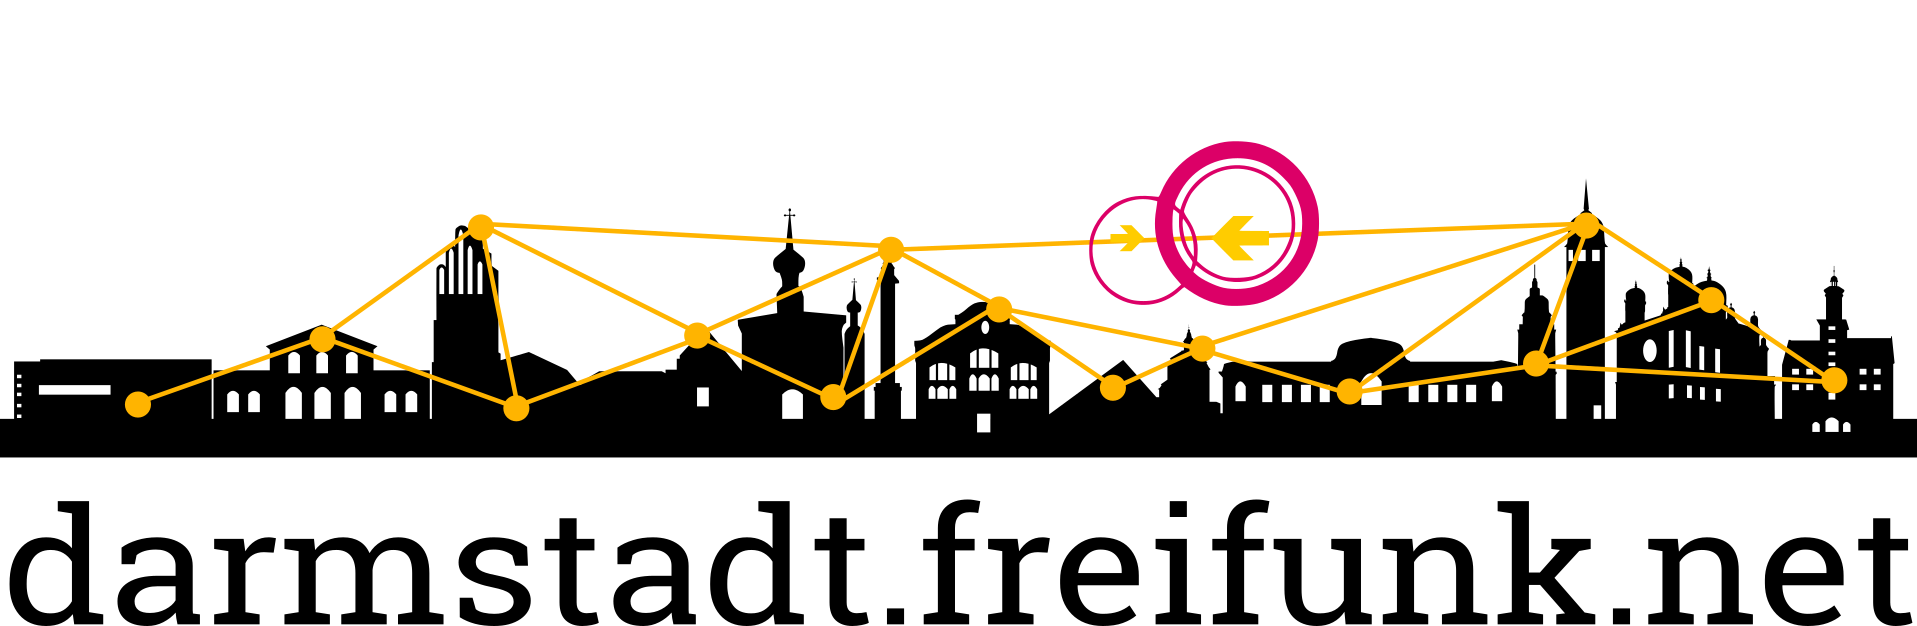
\includegraphics[width=0.6\textwidth]{images/logo-skyline-text-below}
			\vspace{1.4cm}
		\end{center}
			\flushright
			
\includegraphics[width=0.15\textwidth]{images/cda}
	\end{titleframe}
	
	\begin{frame}
		\frametitle{Einleitung}
		\vfill
		\textbf{Was ist Freifunk?}
		\vfill
		\begin{itemize}
			\item nichtkommerzielle Initiative
			\item Ziel: Aufbau und Betrieb eines freien WLAN-Meshnetzes
			\item dezentrales Netz besteht aus den Routern vieler einzelner Betreiber
			\item ca. 20.000 Freifunk-Router in Deutschland
			\item OpenWrt basierte Firmware von Enthusiasten in den Communities vor Ort entwickelt
		\end{itemize}
		\vfill
		\pause
		Um unkompliziert eigene Services im Freifunk-Netz anbieten zu können, soll im Rahmen dieses Projekts ein Dienst erstellt werden, der das Publizieren und Entdecken verfügbarer Services für den Knoten-Betreiber übernimmt.		
	\end{frame}

	\begin{frame}
		\frametitle{Die Idee}
		\vfill
		Hier sehen Sie eine tolle Grafik...
		\vfill
	\end{frame}
	
	\begin{frame}
		\frametitle{Aufgabenstellung (1/2)}
		    Entwicklung eines Publish- und Auto-Discovery-Dienstes, welcher lokal auf Freifunk-Routern ausgeführt wird.
		    \vfill
		    \pause
		    Zusätzlich werden folgende Komponenten benötigt:
		    \begin{itemize}
		    	\item angebotene Dienste dem nächsten Freifunk-Router melden
		    	\item ein zentrales Dienstverzeichnis
		    \end{itemize}
		    \vfill
		    \pause
		    Zur Unterstützung der Entwicklung und für Funktionstests werden zwei Router mit Freifunk-Firmware bereitgestellt.
	\end{frame}
	
	\begin{frame}
		\frametitle{Aufgabenstellung (2/2)}
		\vfill
		Vorgaben zur Realisierung
		\begin{itemize}
			\item als Programmiersprache C oder C++
			\item Paketierung für OpenWRT-basierte Systeme (OPKG)
			\item unter Revisionskontrolle mit Git und sprechenden Commit-Messages\footnote{vgl. \url{http://chris.beams.io/posts/git-commit/}}
			\item lizensiert unter MIT, LGPL oder vergleichbaren Lizenzen
		\end{itemize}
		\vfill
		\pause
		Die Kommunikation zwischen Router und Server, sowie der Router untereinander soll über wohldefinierte, leicht erweiterbare und gut dokumentierte Schnittstellen erfolgen.
		\vfill
	\end{frame}
	
	\begin{frame}
		\frametitle{Fragen?}
		    \vfill
	\end{frame}

\end{document}